% pet_pbt_talk.tex — CRYSP in-room PET for proton-therapy range verification.
% Talk for a medical-institute audience (physicians, potential collaborators).
% Figures in latex/figs/. Compile: pdflatex pet_pbt_talk.tex (x2 for the outline).
\documentclass[aspectratio=169,11pt]{beamer}

\usepackage[T1]{fontenc}
\usepackage[utf8]{inputenc}
\usepackage{helvet}
\usepackage{graphicx}
\usepackage{booktabs}
\usepackage{amsmath}
\usepackage{tikz}
\usepackage{eurosym}
\usetikzlibrary{shapes.geometric, arrows.meta, positioning, backgrounds}

\graphicspath{{figs/}}

% ---- clean custom look (no external theme needed) --------------------------
\usetheme{default}
\setbeamertemplate{navigation symbols}{}
\definecolor{crBlue}{RGB}{22,88,138}
\definecolor{crRed}{RGB}{200,74,40}
\definecolor{crGrey}{RGB}{90,95,100}
\setbeamercolor{title}{fg=crBlue}
\setbeamercolor{frametitle}{fg=crBlue}
\setbeamercolor{structure}{fg=crBlue}
\setbeamercolor{normal text}{fg=black}
\setbeamerfont{frametitle}{series=\bfseries, size=\large}
\setbeamerfont{title}{series=\bfseries}
\setbeamertemplate{itemize item}{\color{crRed}\textbullet}
\setbeamertemplate{itemize subitem}{\color{crGrey}--}
\setbeamertemplate{frametitle}{%
  \vspace{3mm}\hspace{2mm}%
  {\usebeamerfont{frametitle}\usebeamercolor[fg]{frametitle}\insertframetitle}\par
  \hspace{2mm}{\color{crBlue}\rule{0.965\paperwidth}{1.1pt}}\vspace{-1mm}}
\setbeamertemplate{footline}{%
  \hbox{}\hfill{\color{crGrey}\scriptsize\insertframenumber\,/\,\inserttotalframenumber}%
  \hspace{3mm}\vspace{2mm}}

\newcommand{\OT}{\textsuperscript{15}O}
\newcommand{\CE}{\textsuperscript{11}C}
\newcommand{\hi}[1]{\textcolor{crRed}{#1}}

\title[CRYSP in-room PET for PBT]{A High-Sensitivity In-Room \textbf{CRYSP} Scanner\\
  for Distal-Edge Verification in Proton Therapy}
\author{J.J.\ G\'omez-Cadenas, F.\ L\'opez-Guejo and R.\ Soleti}
\date{\small BioGipuzkoa \\ \today}

\begin{document}

{\setbeamertemplate{footline}{}
\begin{frame}[plain]
  \titlepage
\end{frame}}

% ===========================================================================
\section{PET for proton therapy}

\begin{frame}{Proton therapy: a sharp tool that must be aimed precisely}
  \begin{columns}[T]
    \begin{column}{0.56\textwidth}
      \begin{itemize}
        \item Protons deposit most of their dose near the end of their path:
          the \hi{Bragg peak}.
        \item The sharp \hi{distal falloff} spares tissue beyond the tumour,
          but makes the treatment sensitive to range errors.
        \item A few millimetres can mean tumour underdose or damage to a nearby
          critical organ.
        \item For the 10\,cm nominal range shown here,
          \hi{$3.5\%\times\text{range}\simeq3.5$\,mm} uncertainty arises from
          the CT conversion alone.
      \end{itemize}
    \end{column}
    \begin{column}{0.44\textwidth}
      \centering
      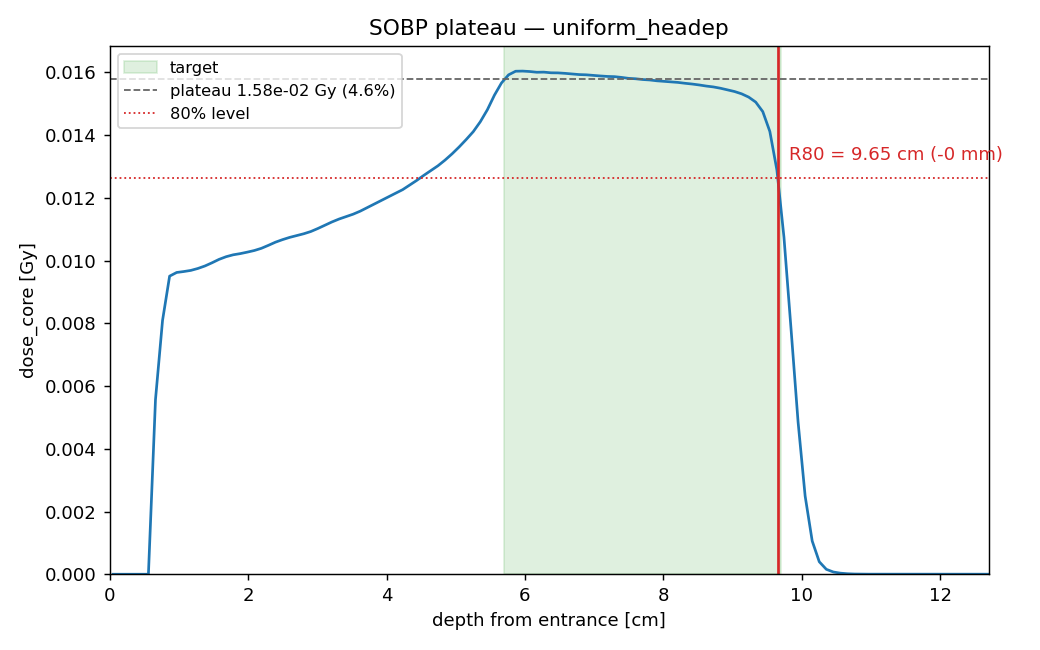
\includegraphics[width=\linewidth]{sobp_plateau.png}\\
      {\scriptsize\color{crGrey} Spread-out Bragg peak (SOBP): flat dose over the
       tumour, sharp distal edge.}
    \end{column}
  \end{columns}
\end{frame}

\begin{frame}{PET: an \emph{in vivo} probe of where the beam stopped}
  \begin{columns}[T]
    \begin{column}{0.54\textwidth}
      \begin{itemize}
        \item Above the nuclear-reaction threshold, protons create
          \hi{$\beta^+$ emitters} along their path --- mainly \OT\ and \CE.
        \item Their annihilation $\gamma$'s are imaged in coincidence: a PET
          image of the \hi{induced activity}.
        \item The activity falloff sits just upstream of the Bragg peak; its
          \hi{distal edge tracks the range}.
      \end{itemize}
    \end{column}
    \begin{column}{0.46\textwidth}
      \centering
      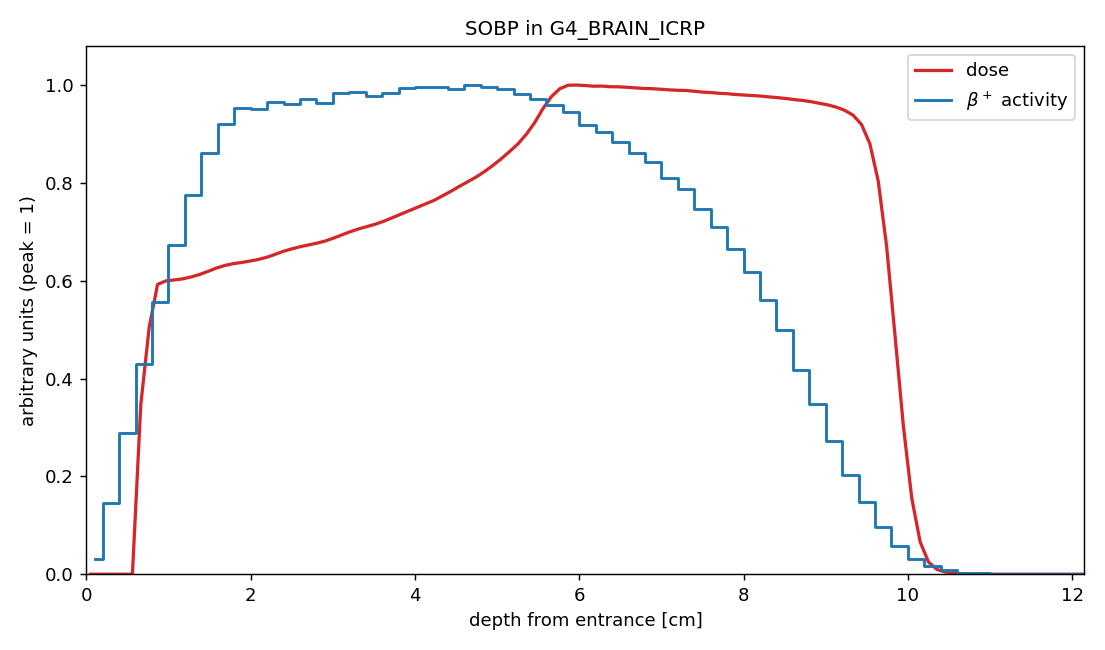
\includegraphics[width=\linewidth]{dose_activity.png}\\
      {\scriptsize\color{crGrey} Dose (Bragg peak) vs.\ $\beta^+$ activity and its
       distal edge.}
    \end{column}
  \end{columns}
\end{frame}

\begin{frame}{PET in proton therapy in brain}
  \begin{columns}[T]
    \begin{column}{0.58\textwidth}
      \begin{itemize}
        \item \hi{Rigid, reproducible positioning} --- the target sits in the
          same place every fraction.
        \item Compact, well-defined anatomy: a \hi{short field of view} covers
          it comfortably.
        \item High clinical stakes: paediatric and skull-base tumours next to
          critical structures.
        \item Our illustrative case: a \hi{fourth-ventricle ependymoma}.
      \end{itemize}
    \end{column}
    \begin{column}{0.42\textwidth}
      \centering
      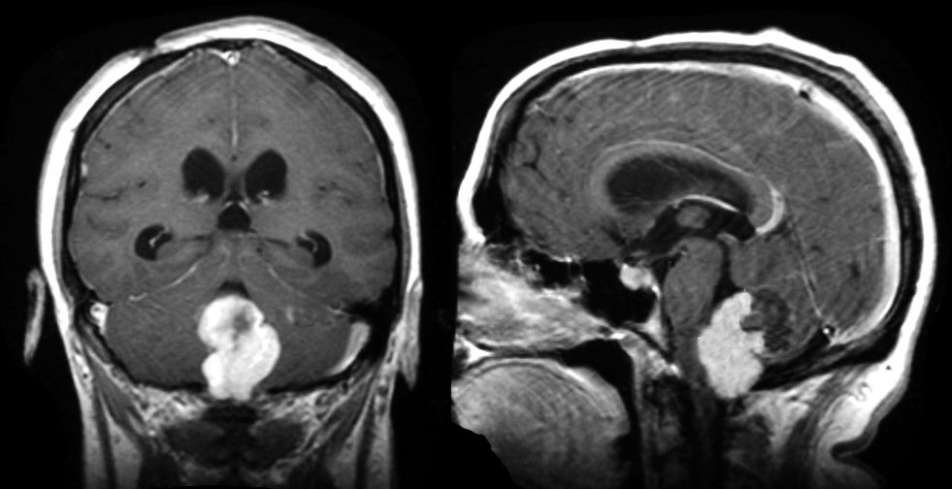
\includegraphics[height=0.42\textheight]{ependymoma_mri.png}\\
      {\scriptsize\color{crGrey} Fourth-ventricle ependymoma (MRI).}
    \end{column}
  \end{columns}
\end{frame}

\begin{frame}{Head phantom used in the simulation}
  \centering
  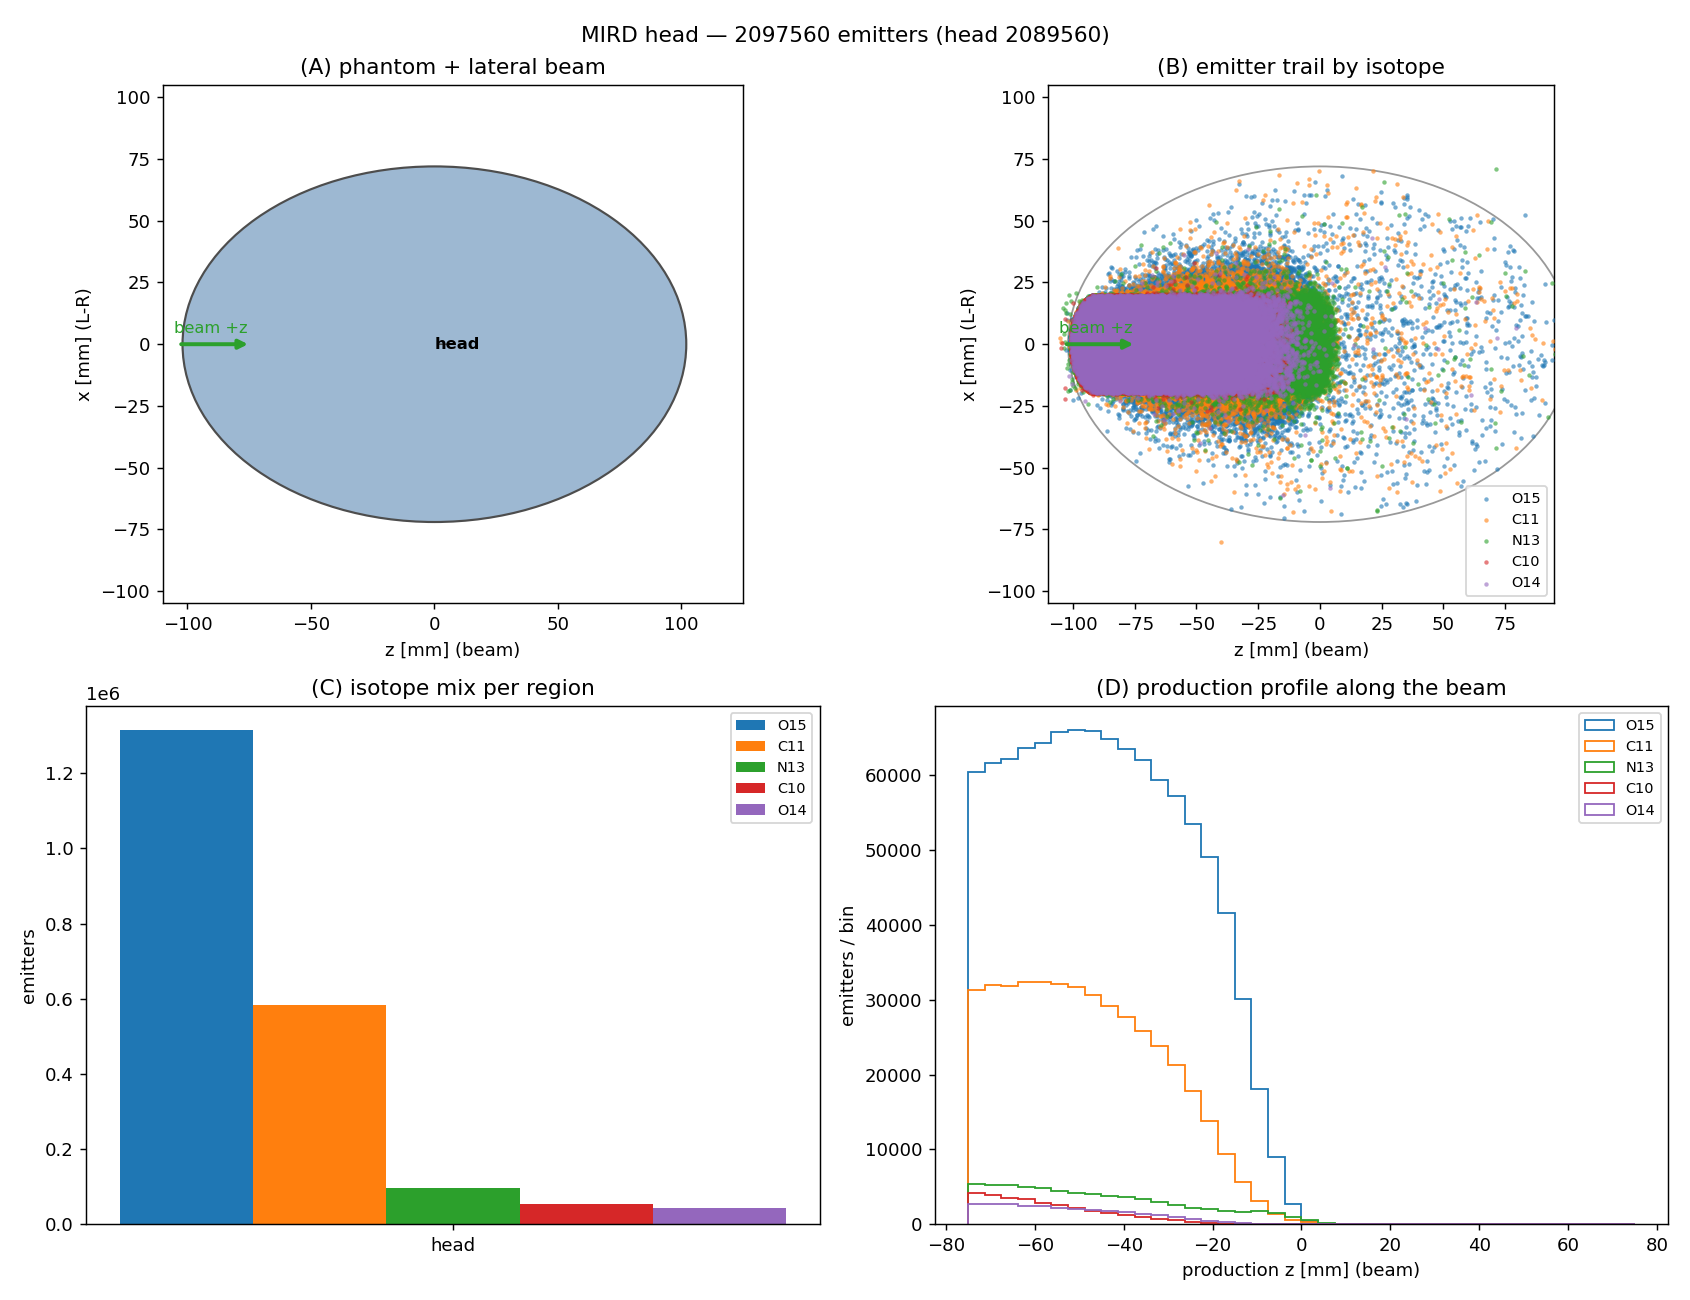
\includegraphics[height=0.82\textheight]{mird_head.png}
\end{frame}

% ===========================================================================
\section{State of the art}

\begin{frame}{PET range verification: offline, in-beam and in-room}
  \centering
  
\includegraphics[width=0.94\textwidth,height=0.80\textheight,keepaspectratio]{in-room.png}
\end{frame}

\begin{frame}{PET range verification: offline, in-beam and in-room}
  \centering
  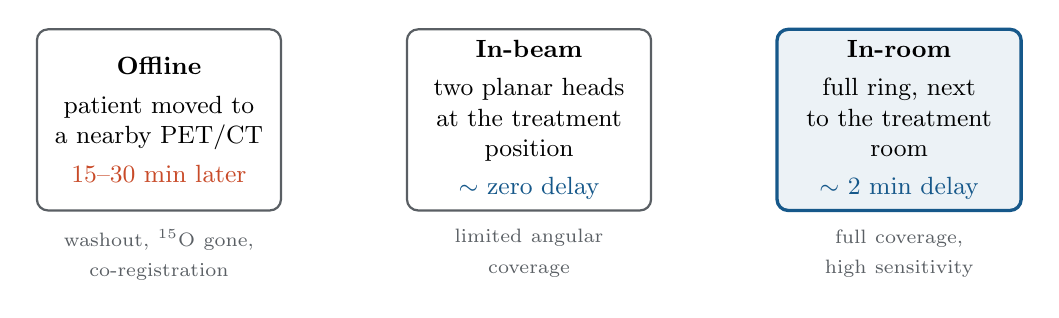
\begin{tikzpicture}[font=\small, node distance=6mm]
    % offline
    \node[draw=crGrey, rounded corners, minimum width=3.1cm, minimum height=2.3cm,
          align=center, thick] (off) at (0,0)
      {\textbf{Offline}\\[1mm] patient moved to\\ a nearby PET/CT\\[1mm]
       \textcolor{crRed}{15--30 min later}};
    % in-beam
    \node[draw=crGrey, rounded corners, minimum width=3.1cm, minimum height=2.3cm,
          align=center, thick] (ib) at (4.7,0)
      {\textbf{In-beam}\\[1mm] two planar heads\\ at the treatment\\ position\\[1mm]
       \textcolor{crBlue}{$\sim$ zero delay}};
    % in-room
    \node[draw=crBlue, fill=crBlue!8, rounded corners, minimum width=3.1cm,
          minimum height=2.3cm, align=center, very thick] (ir) at (9.4,0)
      {\textbf{In-room}\\[1mm] full ring, next\\ to the treatment\\ room\\[1mm]
       \textcolor{crBlue}{$\sim$ 2 min delay}};
    \node[below=1mm of off, text width=3.1cm, align=center, crGrey]
      {\scriptsize washout, \OT\ gone,\\ co-registration};
    \node[below=1mm of ib, text width=3.1cm, align=center, crGrey]
      {\scriptsize limited angular\\ coverage};
    \node[below=1mm of ir, text width=3.1cm, align=center, crGrey]
      {\scriptsize full coverage,\\ high sensitivity};
  \end{tikzpicture}
  \vspace{2mm}

  {\color{crGrey}\small The trade-off is \textbf{delay} vs.\ \textbf{angular
   coverage / scanner quality}.}
\end{frame}

\begin{frame}{Offline results in large uncertainties}
  \begin{columns}[T]
    \begin{column}{0.56\textwidth}
      A delay of 15--30 minutes costs on three fronts:
      \begin{itemize}
        \item \hi{Sensitivity}: the abundant \OT\ (2\,min) has vanished --- only
          the sparse \CE\ tail remains.
        \item \hi{Biological washout}: perfusion clears the emitters; hard to
          model, patient-dependent.
        \item \hi{Co-registration}: the patient is set up afresh on a separate
          scanner --- a few-mm misalignment maps straight into an apparent
          range shift.
      \end{itemize}
      \vspace{1mm}
%      {\small\color{crGrey} Literature: offline accuracy a few mm at best
%       (Knopf 2009; Parodi).}
    \end{column}
    \begin{column}{0.44\textwidth}
      \centering
      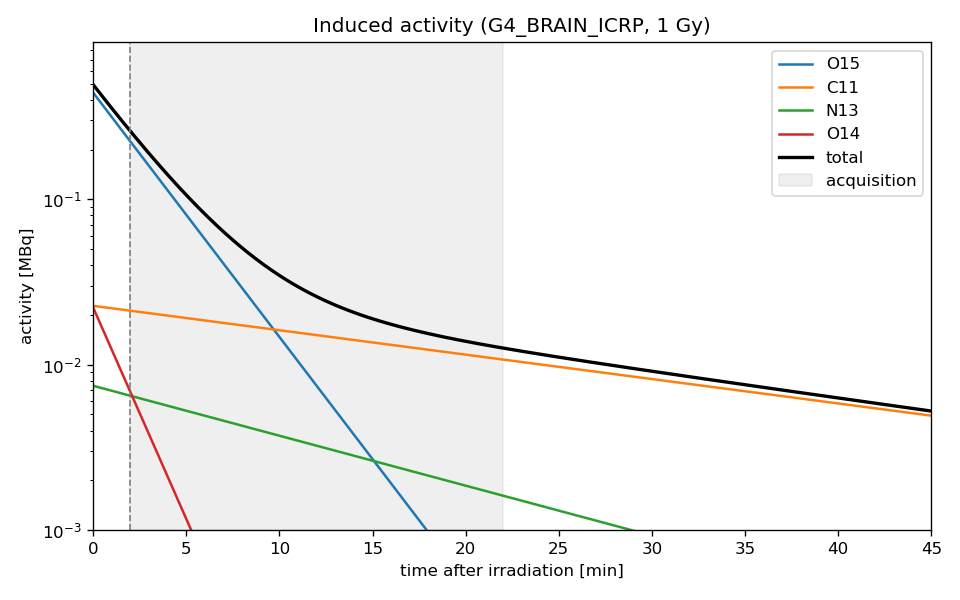
\includegraphics[width=\linewidth]{activity.png}\\
      {\scriptsize\color{crGrey} \OT\ dominates the first minutes, then decays;
       \CE\ carries the late, weak signal.}
    \end{column}
  \end{columns}
\end{frame}

\begin{frame}{Online/In-room tradeoffs}
  \begin{columns}[T]
    \begin{column}{0.5\textwidth}
      \textbf{\color{crBlue}In-beam} (short delay, same bed)
      \begin{itemize}
        \item Retains the short-lived \OT, essentially no delay.
        \item But the beam must pass: only \hi{two planar heads} fit.
        \item Reduced angular coverage $\Rightarrow$ \hi{low sensitivity} and
          limited-angle image artefacts.
      \end{itemize}
    \end{column}
    \begin{column}{0.5\textwidth}
      \textbf{\color{crBlue}In-room} (just after, full ring)
      \begin{itemize}
        \item A \hi{full closed ring} $\Rightarrow$ full coverage, high
          sensitivity, clean image.
        \item Same room $\Rightarrow$ \hi{no co-registration}, short transfer.
        \item The $\sim$2-min delay is \hi{bought back} by sensitivity and a
          \hi{better scanner}.
      \end{itemize}
    \end{column}
  \end{columns}
  \vspace{2mm}
  \begin{center}
    \fbox{\parbox{0.9\textwidth}{\centering
      A \hi{high-sensitivity in-room ring} turns the delay from a liability into
      an opportunity --- and lets us build the scanner we actually want.}}
  \end{center}
\end{frame}

% ===========================================================================
\section{CRYSP}

\begin{frame}{CRYSP: \emph{CRYogenic Sensitive PET}}
  \begin{columns}[T]
    \begin{column}{0.6\textwidth}
      \begin{itemize}
        \item Scintillators \hi{CsI and BGO} gain dramatically in light yield
          when cooled --- CsI reaches $\sim$100 photons/keV at 77 K, BGO $\sim$100 photons/keV.
            \item In both cases, high yields translate into excellent energy resolution
              (6\% CsI, 10\% BGO),
              which in turn is essential for efficient scatter rejection.
            \item Monolithic crystals + SiPMs, permit 3D position reconstruction using neural
              networks with high accuracy and no parallax error. 
      \end{itemize}
  
    \end{column}
    \begin{column}{0.4\textwidth}
      \centering
      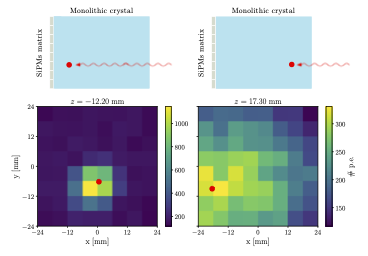
\includegraphics[width=1.08\linewidth]{3D.png}\\
      {\scriptsize\color{crGrey} 3D reconstruction in a monolithic crystal.}
    \end{column}
  \end{columns}
\end{frame}

%\begin{frame}{One concept, a family of scanners}
%  \centering
%  \begin{tabular}{lccc}
%    \toprule
%    Configuration & Axial FOV & Inner radius & Role \\
%    \midrule
%    \textbf{TBP} (reference)   & 1024\,mm & 387\,mm & total-body reach \\
%    \textbf{LAFOV}             & 512\,mm  & 350\,mm & most indications \\
%    \textbf{CAFOV}             & 358\,mm  & 350\,mm & head / skull-base \\
%    \bottomrule
%  \end{tabular}
%  \vspace{3mm}
%  \begin{itemize}
%    \item Monolithic CsI or BGO, $48\times48$\,mm$^2$, 2 radiation lengths deep.
%    \item Head and skull-base targets fit the \hi{compact} configuration ---
%      cheaper, and enough.
%    \item Longer axes buy sensitivity and reach for craniospinal / body sites.
%  \end{itemize}
%\end{frame}

\begin{frame}{Scanner cost breakdown}
  \centering
  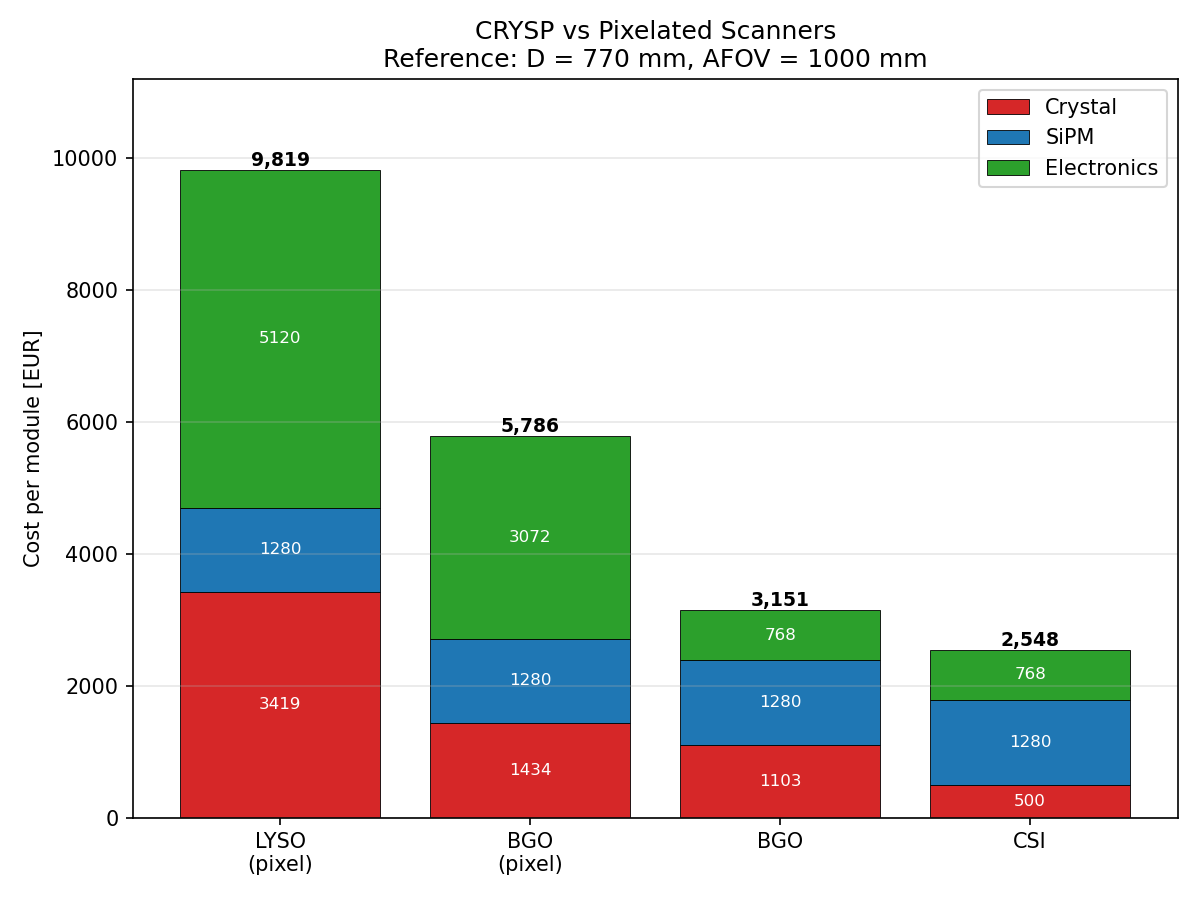
\includegraphics[width=0.94\textwidth,height=0.80\textheight,keepaspectratio]{cost_breakdown.png}
\end{frame}

\begin{frame}{Total scanner cost}
  \centering
  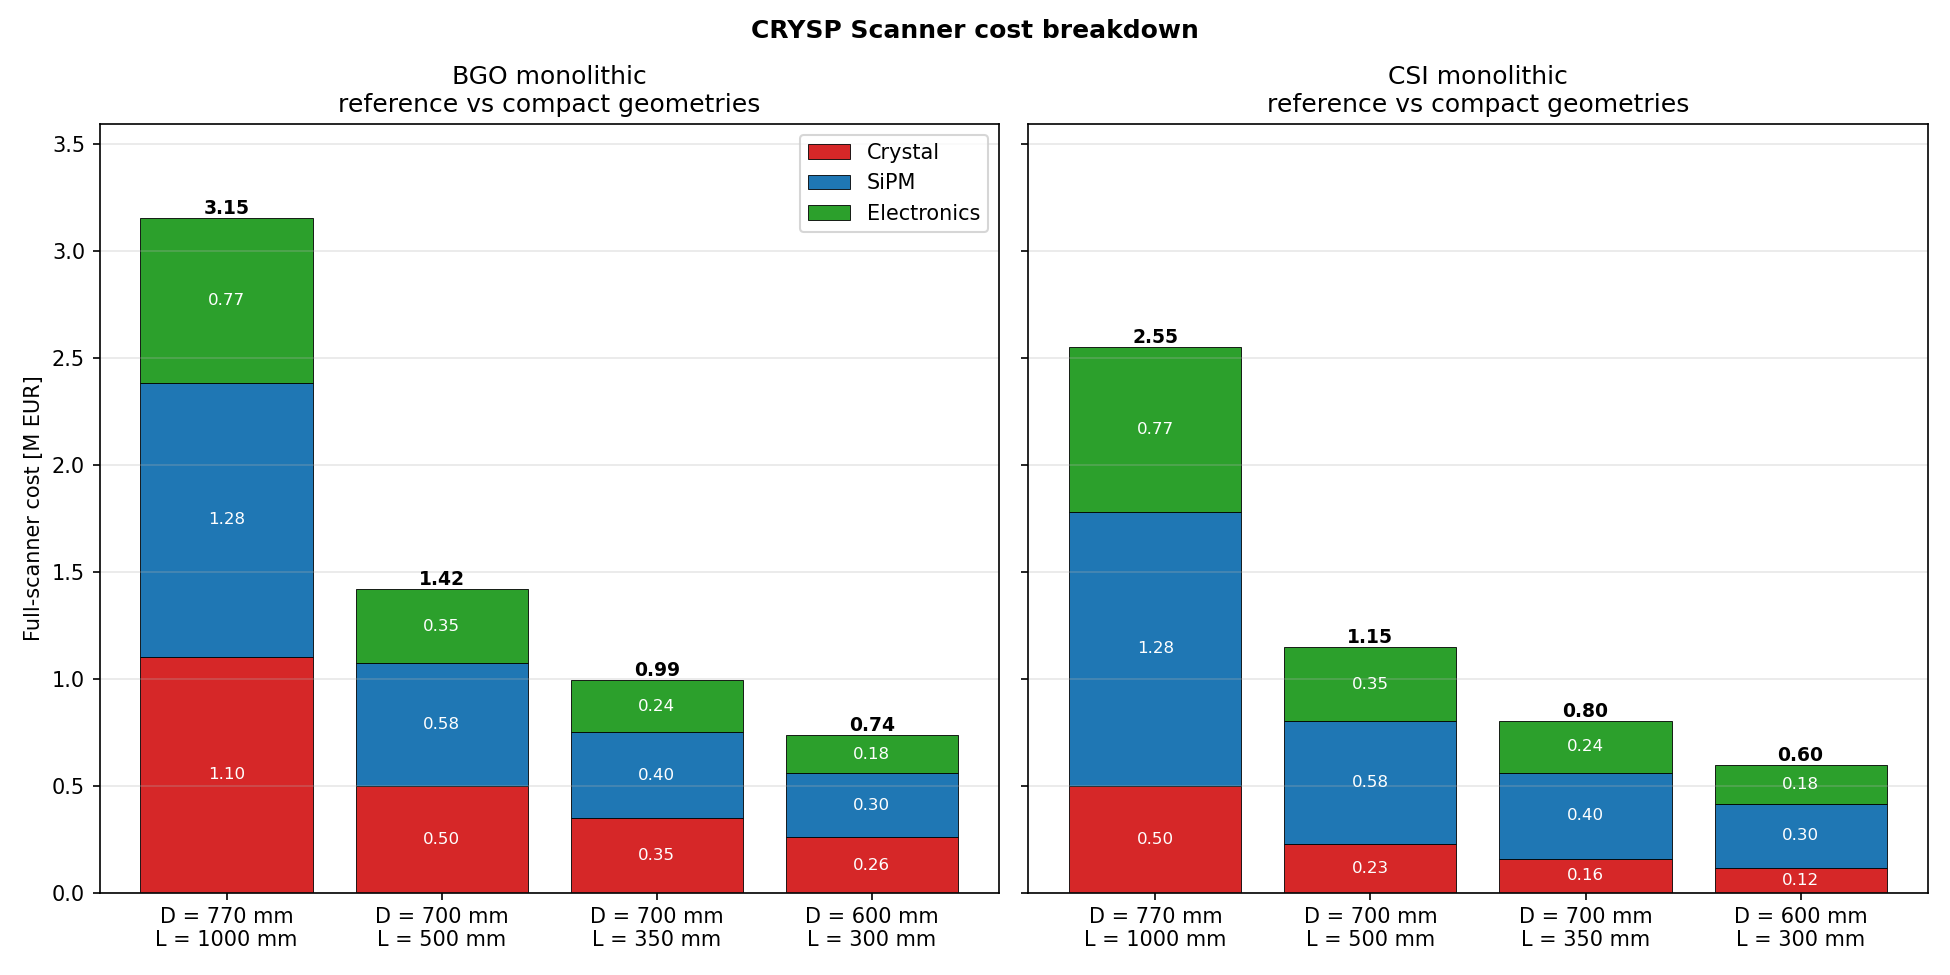
\includegraphics[width=0.94\textwidth,height=0.80\textheight,keepaspectratio]{scanner_totals.png}
\end{frame}

% ===========================================================================
\section{Results}

\begin{frame}{Imaging the brain}
  \centering
  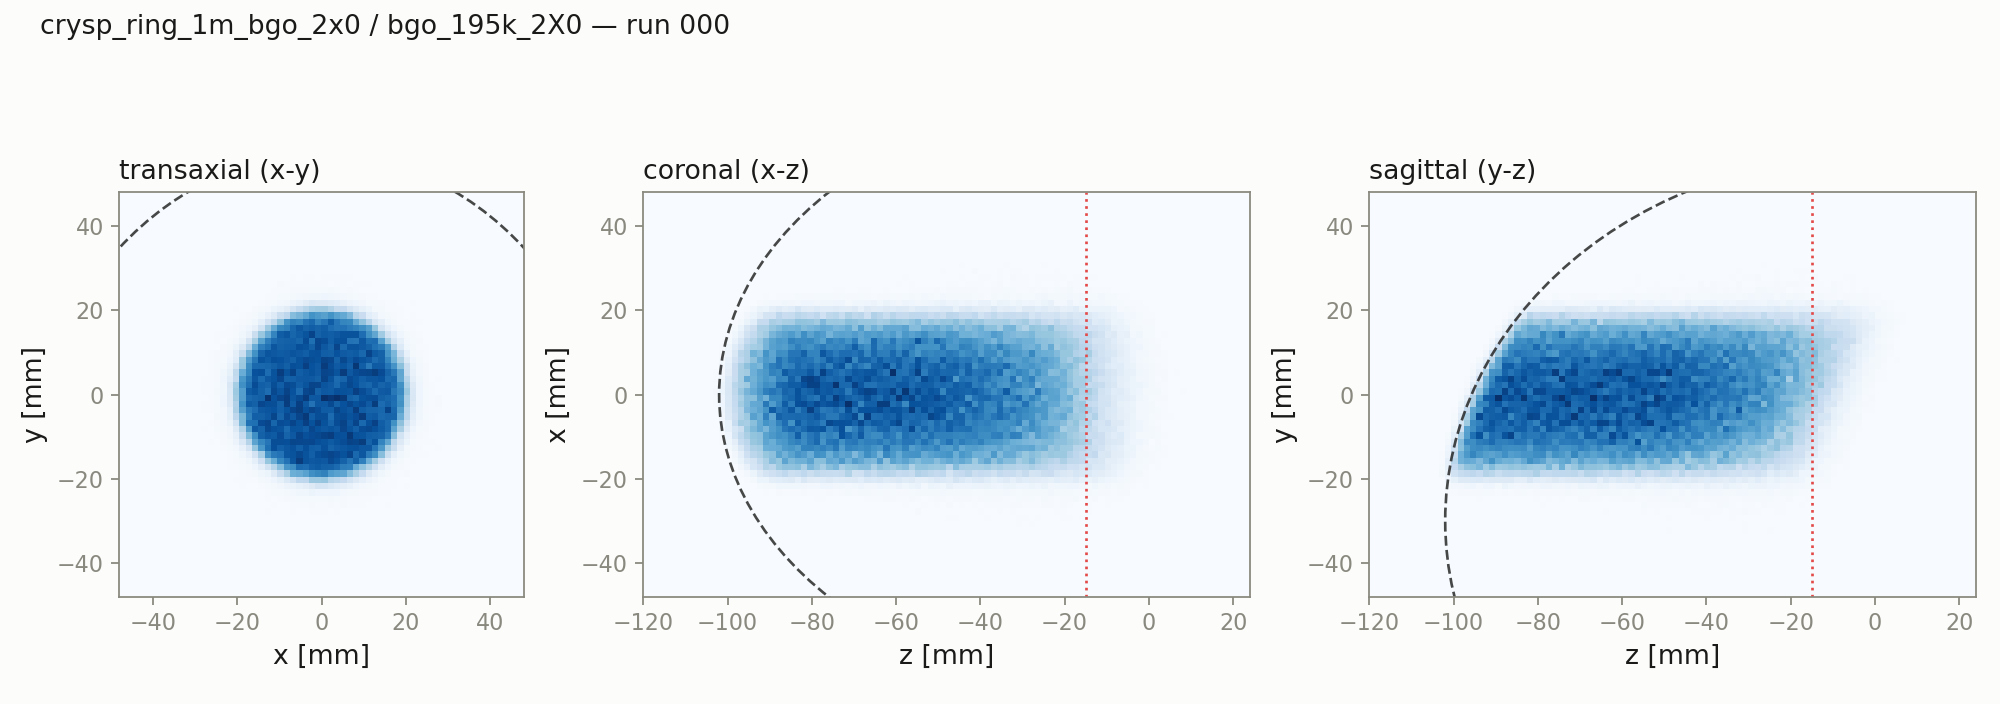
\includegraphics[width=0.88\textwidth,height=0.36\textheight,keepaspectratio]{recon_projections_bgo.png}\\[2mm]
  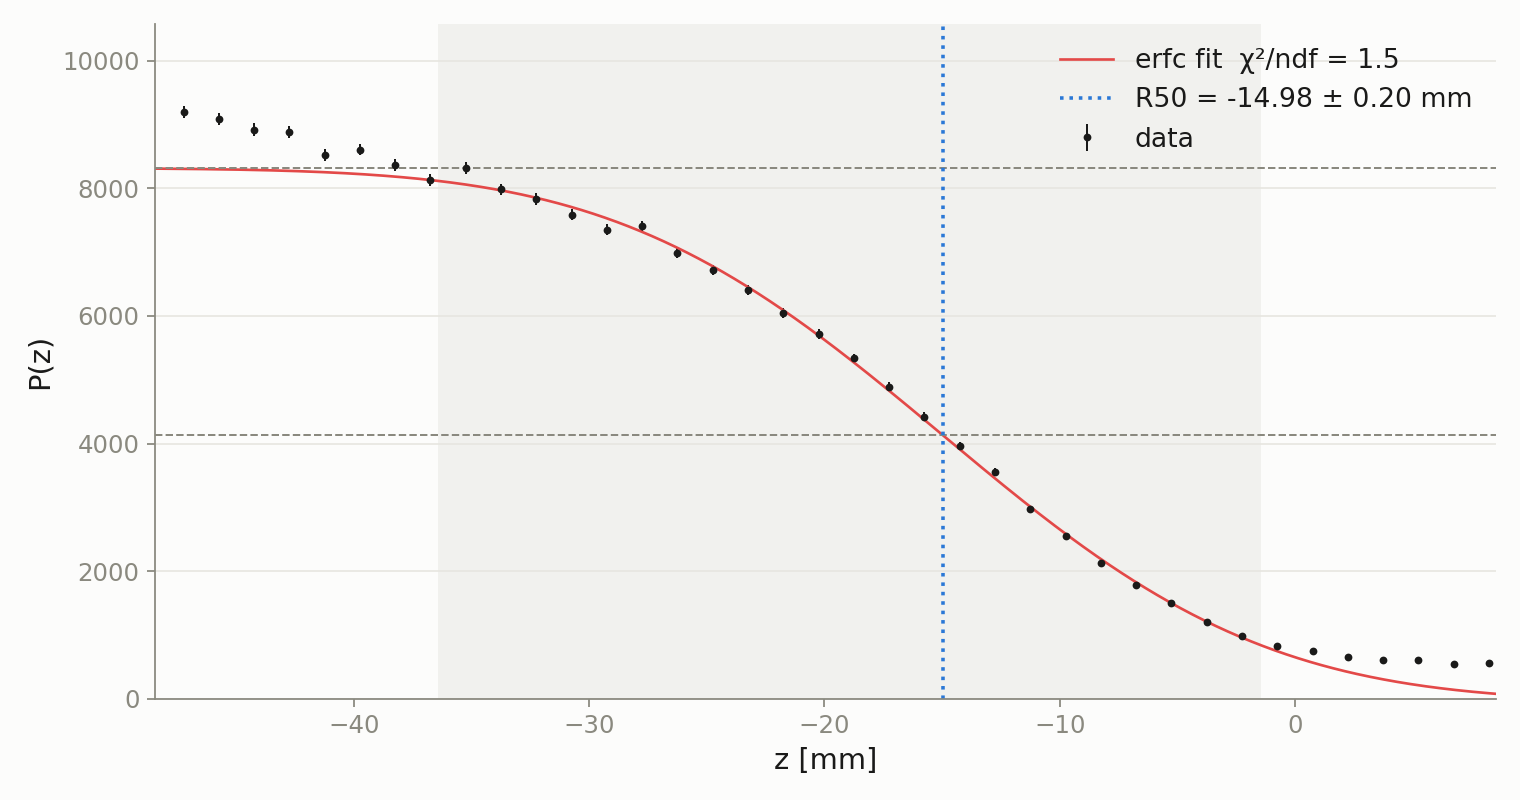
\includegraphics[width=0.88\textwidth,height=0.36\textheight,keepaspectratio]{fit_all_events_bgo.png}
\end{frame}

\begin{frame}{CRYSP can achieve high precision in distal edge determination}
  \begin{columns}[T]
    \begin{column}{0.52\textwidth}
      \begin{itemize}
        \item A single short in-room scan (1\,Gy) locates the distal edge to
          \hi{$\sigma_R \approx 0.15$--$0.3$\,mm} --- well inside clinical
          margins.
        \item \hi{Both crystals perform very well}: BGO ahead on raw
          sensitivity, CsI close behind at lower cost.
        \item Biological washout costs only \hi{$\sim 1.5\times$} in precision,
          with \hi{no range bias}.
        \item Precision holds across scanner sizes and the realistic 2-min
          acquisition delay.
      \end{itemize}
    \end{column}
    \begin{column}{0.48\textwidth}
      \centering
      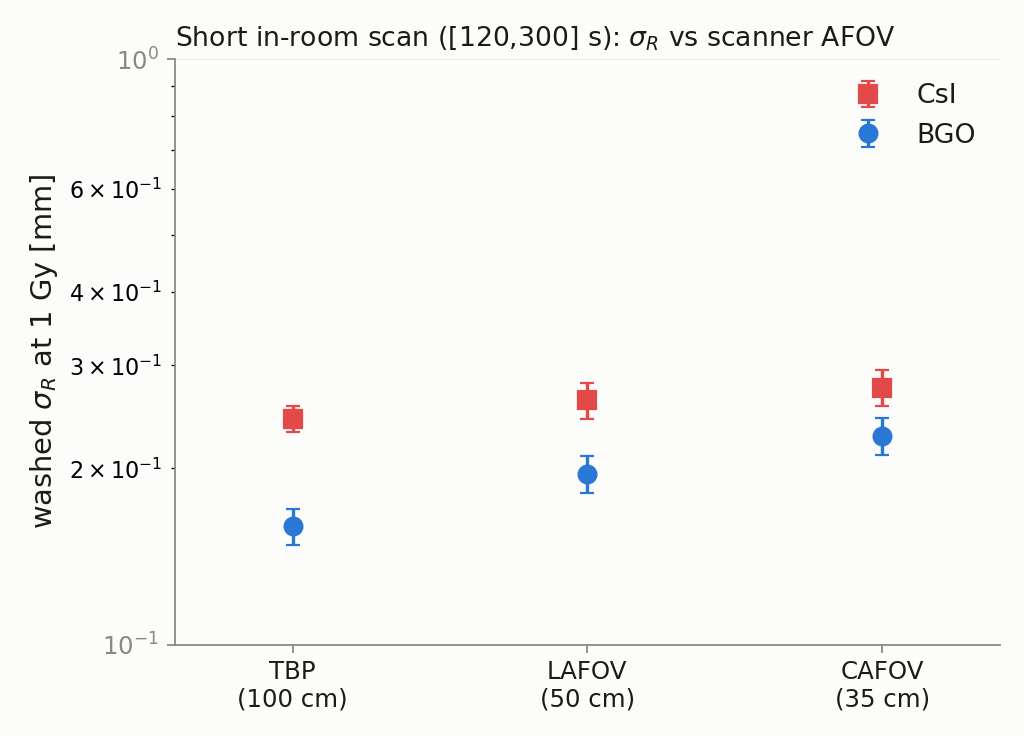
\includegraphics[width=\linewidth]{washed_shortscan_afov.png}\\
      {\scriptsize\color{crGrey} $\sigma_R$ (short in-room scan, with washout)
       vs.\ scanner size, CsI and BGO.}
    \end{column}
  \end{columns}
\end{frame}

%\begin{frame}{Robust across configuration and timing}
%  \begin{columns}[T]
%    \begin{column}{0.5\textwidth}
%      \centering
%      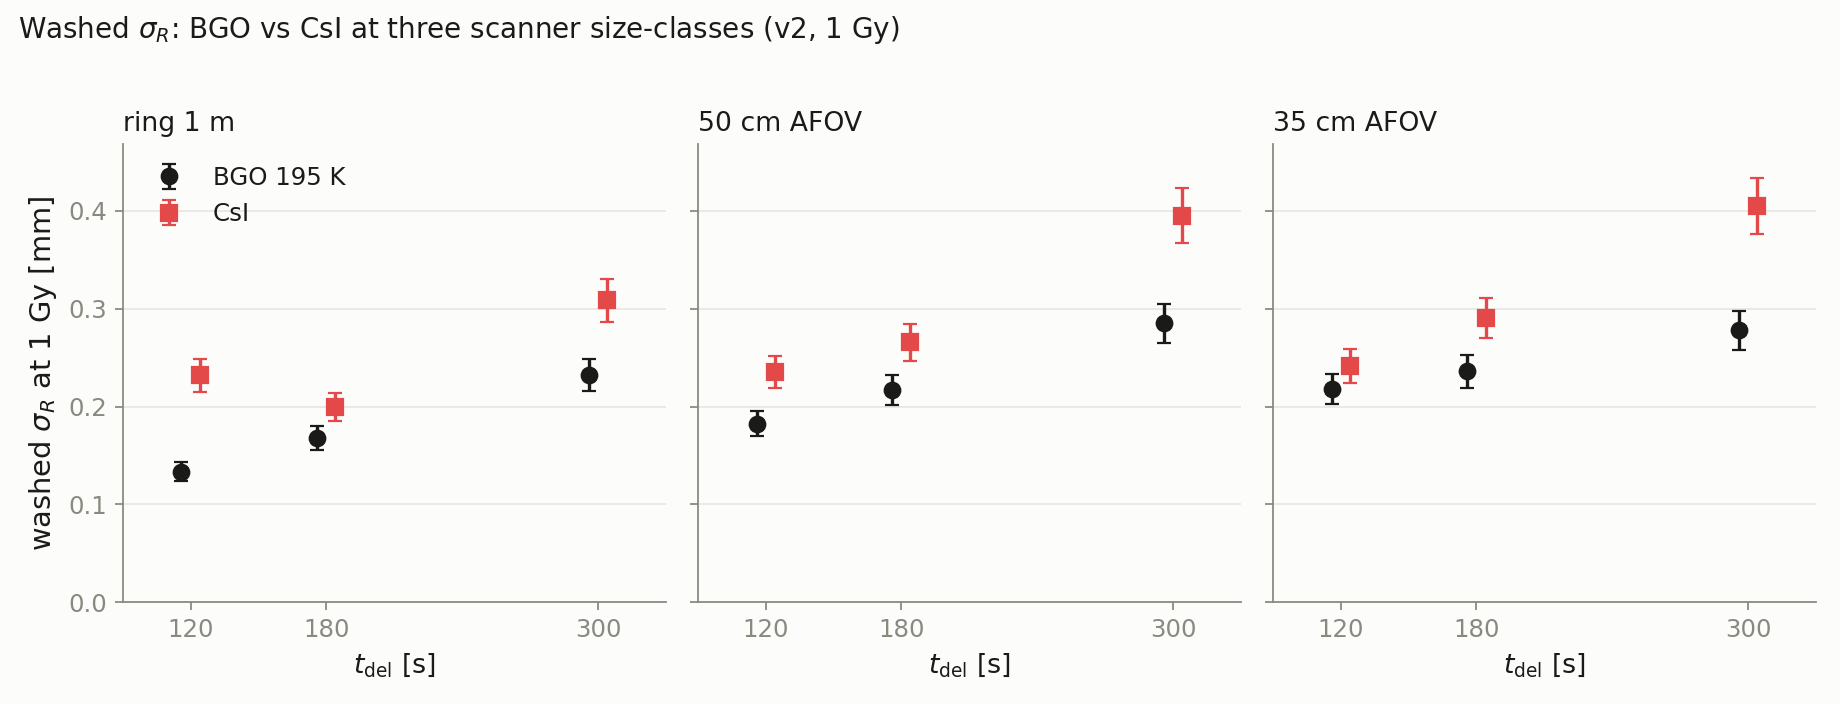
\includegraphics[width=\linewidth]{washed_bgo_vs_csi_v2.png}\\
%      {\scriptsize\color{crGrey} BGO vs.\ CsI at three scanner sizes.}
%    \end{column}
%    \begin{column}{0.5\textwidth}
%      \centering
%      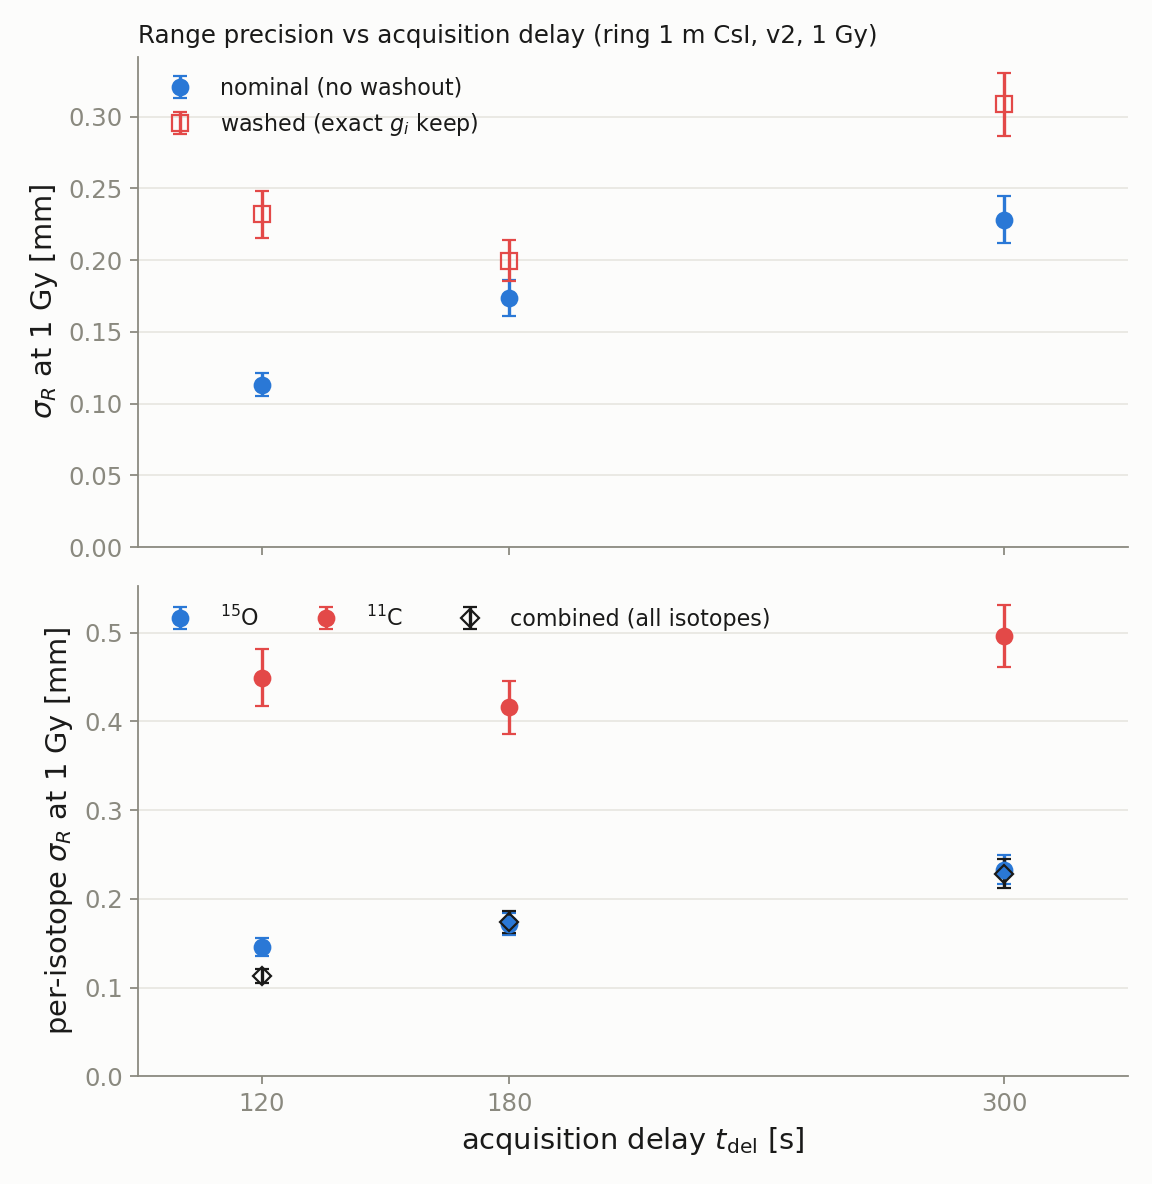
\includegraphics[width=\linewidth]{sigma_r_v2_csi.png}\\
%      {\scriptsize\color{crGrey} Precision vs.\ acquisition delay (CsI).}
%    \end{column}
%  \end{columns}
%  \vspace{1mm}
%  \begin{center}
%    {\color{crGrey}\small The measurement degrades gracefully with delay and
%     scanner size --- and stays sub-mm.}
%  \end{center}
%\end{frame}

% ===========================================================================
\section{Summary}

\begin{frame}{Summary}
  \begin{itemize}
    \item Proton-therapy range verification needs an \hi{in vivo}, online/in-room,
      high-sensitivity probe 
    \item \hi{CRYSP in-room PET} exploits cryogenic CsI/BGO for excellent energy
      and spatial resolution at a \hi{competitive cost}.
    \item On the brain --- the ideal first application --- \hi{both CsI and BGO}
      locate the distal edge to \hi{$\sim 0.15$--$0.3$\,mm} per 1\,Gy scan,
      washout included.
    \item CsI offers a very good, low-cost, supply-secure option; BGO offers the
      best raw performance.
  \end{itemize}
  \vspace{3mm}
\end{frame}

{\setbeamertemplate{footline}{}
\begin{frame}[plain]
  \centering
  {\color{crBlue}\Large Thank you}\\[3mm]
  {\color{crGrey} Questions --- and collaborations --- welcome.}
\end{frame}}

\end{document}
